\chapter{Materials and Methodology}
\section{System Design}
\paragraph{} The system deals with fetching, summarization and creation of front end results for the user. We have used extensive use of python libraries to aid us in parsing data from RSS feeds and extracting data from websites. 
\paragraph{} Next stage was to cluster the documents fetched based on the topics. So we're able to generate input documents for the summarizer. The summarizer using the below mentioned algorithms and methods generate a summery based on length specified. Finally a JSON file is generated for the generated summaries. 
\paragraph{} An HTML front end using AJAX is used to fetch this JSON file to the user. The block diagram given below will make the whole procedure clearer.
\newpage
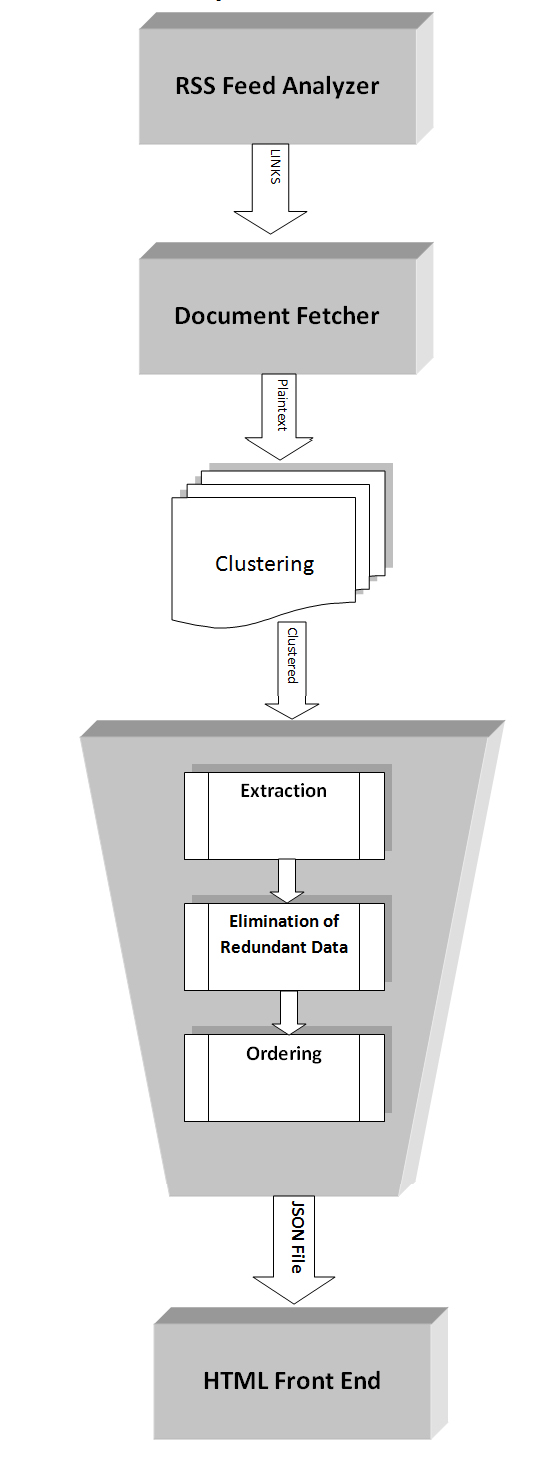
\includegraphics[scale=0.4]{my/images/gh}
\subsection{RSS Feed Analyzer}
\paragraph{} Really Simple Syndication (RSS) is a family of web feed formats used to publish frequently updated works—such as blog entries, news headlines, audio, and video—in a standardized format. It is universally used by news websites for providing news headlines and links to clients. We use a python library developed by Leonard Richardson knows as BeautifulSoup\cite{BeautifulSoup}. It is used to extract tags from the feed page.
\begin{lstlisting}
<xml version="1.0" encoding="UTF-8" >
<rss version="2.0">
<channel>
 <title>RSS Title</title>
 <description>This is an example of an RSS feed</description>
 <link>http://www.someexamplerssdomain.com/main.html</link>
 <lastBuildDate>Mon, 06 Sep 2010 00:01:00 +0000 </lastBuildDate>
 <pubDate>Mon, 06 Sep 2009 16:45:00 +0000 </pubDate>
 <ttl>1800</ttl>
 
 <item>
  <title>Example entry</title>
  <description>Here is some text containing an interesting description.</description>
  <link>http://www.wikipedia.org/</link>
  <guid>unique string per item</guid>
  <pubDate>Mon, 06 Sep 2009 16:45:00 +0000 </pubDate>
 </item>
\end{lstlisting}
\subsection{Document Fetcher}
\paragraph{}Document fetcher is used for fetching articles from the links in the RSS feeds obtained in the above step. Here also we use the above mentioned library BeautifulSoup\cite{BeautifulSoup}. We designed individual fetchers for each site since the HTML framework of each site is different from each other. This was a relatively tiresome task to do.
\paragraph{}	Document Fetcher takes in input as links and gives output as the documents or articles in those links and headings in plain text format. This can be fed into the summarizer as input.
\subsection{Clustering}
\paragraph{} Clustering is used to group large number of documents into clusters. We require this since there would be different news articles fetched from the web and we need to cluster them and group them for generating summery for a group of documents.
\paragraph{}	There are various clustering algorithms available .Old ones include centroid clustering and naïve similarity algorithms. We use the concept of Hierarchical Clustering. Hierarchical clustering is a method of cluster analysis which seeks to build a hierarchy of clusters. Strategies for hierarchical clustering generally fall into two types:
\begin{enumerate}[a. ]
\item \textbf{Agglomerative :} This is a "bottom up" approach: each observation starts in its own cluster, and pairs of clusters are merged as one moves up the hierarchy.
\item \textbf{Divisive :} This is a "top down" approach: all observations start in one cluster, and splits are performed recursively as one moves down the hierarchy.
\end{enumerate}
\begin{equation}
similarity = \cos{\theta} = \frac{A.B}{\|A\|.\|B\|}
\end{equation}
\paragraph{}The choice of an appropriate metric will influence the shape of the clusters, as some elements may be close to one another according to one distance and farther away according to another. We used Cosine Similarity for determining the clusters.
\subsection{Summarization}
\paragraph{} The heart of the project is called the summarizer. This takes in multiple documents and generates the summery based on the given parameters. Multi-document summarization tackles the information overload problem by providing a condensed and coherent version of a set of documents. Among a number of sub-tasks involved in multi-document summarization including sentence extraction, topic detection, sentence ordering, information extraction, and sentence generation, most multi-document summarization systems have been based on an extraction method, which identifies important textual segments (e.g. sentences or paragraphs) in source documents
\subsubsection{Sentense Extraction}
\paragraph{} Sentence extraction is the process of retrieving relevant and non redundant sentences from the document set. We used various methods for implementing this like Cosine Ranking, Centroid Method, and finally the clustering method. In out tests we found out that first method the Cosine Ranking was not very efficient in many cases and was abandoned.
\paragraph{}	The method we use mainly is known as the Centroid method. In this method one aims to create a Centroid of sentences by repeatedly removing the ones with low similarity with the sentence in Centroid and also the ones which have high similarity since they are redundant .This ensures that we get a good set of sentences which are relevant and non redundant.
\begin{lstlisting}
while (n<N)
	for each sentence in documents:
		Find cosine similarity with document vector;
		if( cs  > threshold 1)
			Add sentence to set
		if(cs < threshold2)
			Remove sentence from document 
		n++
	end  for
end while
\end{lstlisting}
\paragraph{} The method that improves the extraction process even more is known as Clustering combined with Centroid .This ensures even better result and more relevant sentences are selected due the initial clustering operation. This is basically grouping a set of objects in such a way that objects in the same group (called cluster) are more similar (in some sense or another) to each other than to those in other groups (clusters)
\subsubsection{Ordering}
\paragraph{} The next important thing to after extraction of sentences is that it needs to be ordered properly so that the user feels continuity while reading. This makes it one of the most complex steps in summarization as a whole since there’s no quantitative way to check the validity of this operation. We can only rely on human verification for this. A summary with improperly ordered sentences both confuses the reader and degrades the quality/reliability of the summary. Study shows that the proper order of extracted sentences significantly improves their readability. It has been experimentally shown that the time taken to read a summary strongly correlates with the arrangement of sentences in the summary.
\paragraph{}	But despite this some probabilistic and chronological methods exist for doing this. We employ 3 such methods here. They are 1) Chronological 2) Precedence 3) Succession. We use these three methods to find the relative rank of a sentence in the summary. Each of this are assigned weights that when varied will produce different weights for each method.
\begin{enumerate}[a. ]
\item \textbf{Chronological Expert :} \newline The author of a particular document is likely to order the sentences logically to make the document coherent. Therefore, for sentences belonging to a particular document, we can safely retain this original order given by the author. In single document summarization this simple ordering strategy is often adequate to order all the extracted sentences because those sentences belong to a single document.

Chronological ordering we use can be summarized by the function 
\begin{equation}
PREF_{chro}(u,v,Q) = \begin{cases}
	1 & T(u) < T(v)\\
	1 & [D(u) = D(v)] \wedge [N(u) < N(v)]\\
	0.5 & [T(u) = T(v)] \wedge [D(u) \neq D(v)]\\
	0 & otherwise
\end{cases} 
\end{equation}
\paragraph{} In the above equation the expert returns 1 if the relative position of the first 	sentence is in front of the second and they both are in the same document. It does the 		same if they are from different documents .It returns the value 0.5 if they both are in 	same position in the document.
\item \textbf{Precedence expert :} In extractive multi-document summarization, only the important sentences that convey the main points discussed in source documents are selected to be included in the summary. However, a selected sentence can presuppose information from other sentences that were not selected by the sentence extraction algorithm.
\begin{equation}
pre(I) = \frac{1}{|Q|}\sum_{q \in Q, p \in Pq}^{N} maxism(p,I)
\end{equation}
\paragraph{} Here the precedence value of a sentence is calculated by taking the maximum cosine similarity of obtained when cosine similarity is calculated for n sentences before that. Finally when two sentences are compared this relation is used.
\begin{equation}
PREF_{pre}(u,v,Q) = \begin{cases}
	0.5 & [Q \neq \emptyset ] \vee [pre(u) = pre(v)]\\
	1 & [Q \neq \emptyset ] \wedge [pre(u) > pre(v)]\\
	0 & otherwise
\end{cases}
\end{equation}
\item \textbf{Succession Expert :} In extractive multi-document summarization, sentences that 	describe a particular event are extracted from a set of source articles.
\begin{equation}
PREF_{succ}(u,v,Q) = \begin{cases}
	0.5 & [Q \neq \emptyset ] \vee [succ(u) = succ(v)]\\
	1 & [Q \neq \emptyset ] \wedge [succ(u) > succ(v)]\\
	0 & otherwise
\end{cases}
\end{equation}
\item Usually, there exists a logical sequence among the information conveyed in the extracted sentences.
\begin{equation}
succ(I) = \frac{1}{|Q|}\sum_{q \in Q, p \in Pq}^{N} maxism(s,I)
\end{equation}
\paragraph{} Here the succession value of a sentence is calculated by taking the 			maximum cosine similarity of obtained when cosine similarity is calculated for n 	sentences after that. Finally when two sentences are compared this relation is used.
\begin{equation}
PREF_{succ}(u,v,Q) = \begin{cases}
	0.5 & [Q \neq \emptyset ] \vee [succ(u) = succ(v)]\\
	1 & [Q \neq \emptyset ] \wedge [succ(u) > succ(v)]\\
	0 & otherwise
\end{cases}
\end{equation}

\end{enumerate}
\subsubsection{Ordering Algorithm}
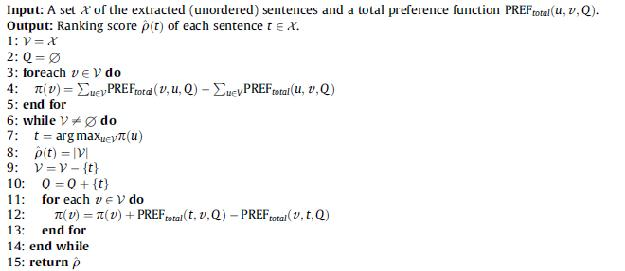
\includegraphics[scale=0.75]{my/images/algorithm}
\paragraph{} Algorithm greedily calculates the most eligible sentence for selection based on the combined effect of these three factors. The sentence so selected is removed from the summary set and the weights / potentials is updated for each vertex to reflect the removal of the sentence. This is repeated for all sentences in the selected set .  


\section{Platform Details}
\subsection{Python}

\paragraph{} Python is a general purpose, high-level programming language whose design philosophy emphasizes code readability. Python's syntax allows programmers to express concepts in fewer lines of code than would be possible in languages such as C and the language provides constructs intended to enable clear programs on both a small and large scale. Python is a programming language that lets you work more quickly and integrate your systems more effectively. Python has small and has clean source codes. Standard library is full of useful modules.
\paragraph{} Python supports multiple programming paradigms, including object-oriented, imperative and functional programming styles. It features a dynamic type system and automatic memory management and has a large and comprehensive standard library.
\paragraph{} Like other dynamic languages, Python is often used as a scripting language, but is also used in a wide range of non-scripting contexts. Using third-party tools, Python code can be packaged into standalone executable programs. Python interpreters are available for many operating systems.
\textbf{Syntax and Semantics}
\paragraph{} The syntax of the Python programming language is the set of rules that defines how a Python program will be written and interpreted (by both the runtime system and by human readers). Python was designed to be a highly readable language. It has a relatively uncluttered visual layout and uses English keywords frequently where other languages use punctuation. Python aims towards simplicity and generality in the design of its syntax.
\paragraph{} Python uses whitespace indentation, rather than curly braces or keywords, to delimit blocks; a feature also termed the off-side rule. An increase in indentation comes after certain statements; a decrease in indentation signifies the end of the current block.
\textbf{Features of Python}
\begin{enumerate}[1. ]
\item \textbf {Simple} \newline Python is a simple and minimalistic language. Reading a good Python program feels like reading English, although very strict English! This pseudo-code nature of Python is one of its greatest strengths.

\item \textbf{Easy to Learn} \newline As we will discover in this book, Python is very easy to get started with and has an extraordinarily simple syntax.
\item \textbf{Free and Open Source} \newline Python is an example of an open source software. In simple terms, you can freely distribute copies of the software, read the source code, make changes to it and use pieces of it in new free programs. Open source is based on the concept of a community which shares knowledge. This is one of the reasons why Python is so good - it is constantly improved by a community which just wants to see a better Python.
\item \textbf{High-level Language} \newline When you write programs in Python, you do not need to bother about low-level details such as managing the memory used by your program, etc.
\item \textbf{Portable} \newline Due to its open source nature, Python has been ported to (i.e. changed to make it work on) many platforms. All your Python programs can work on any of these platforms without requiring any changes as long as you are careful to avoid any system-specific features.
\item \textbf{Interpreted} \newline Python, on the other hand, does not need the compilation and linking/loading steps. You just run the program directly from source code. Internally, Python converts the source program into an intermediate form called bytecodes and then translates this into the native language of your specific system and then runs it. All this actually makes Python much easier to use since you do not have to worry about compiling the program, making sure the proper libraries are linked and loaded, etc. This also makes your Python programs more portable since you can just copy the program to another computer and it just works!
\item \textbf{Object Oriented} \newline Python supports both procedure-oriented programming as well as object-oriented programming. In procedure-oriented programming, the program is built around procedures or functions which are just reusable pieces of programs to which data is fed. In object-oriented programming, the program is built around objects which combine both data and functionality.


\item \textbf{Extensible} \newline If you need a critical piece of code in your program to run very fast or want to have a piece of algorithm to be hidden from the outside world, then you can write that part of the program in languages like C or C++ and then use that part from your Python programs.
\item \textbf{Embeddable} \newline You can embed Python in your programs written in other languages like C or C++ to give 'scripting' capabilities for your program's users.
\item \textbf{Extensive Libraries}
\end{enumerate}
\subsection{NLTK}
\paragraph{} The Python Standard Library is huge. It can help you with regular expressions, documentation generation, unit testing, threading, databases, web browsers, CGI, FTP, email, XML, HTML, WAV files, cryptography, GUI using Tk, and  many other system-specific functionality as well.
\paragraph{} NLTK is a leading platform for building Python programs to work with human language data. It provides easy-to-use interfaces to over 50 corpora and lexical resources such as WordNet, along with a suite of text processing libraries for classification, tokenization, stemming, tagging, parsing, and semantic reasoning.
\paragraph{} Thanks to a hands-on guide introducing programming fundamentals alongside topics in computational linguistics, NLTK is suitable for linguists, engineers, students, educators, researchers, and industry users alike. NLTK is available for Windows, Mac OS X, and Linux. Best of all, NLTK is a free, open source, community-driven project. 
\paragraph{} NLTK has been called “a wonderful tool for teaching, and working in, computational linguistics using Python,” and “an amazing library to play with natural language.”
\paragraph{} Natural Language Processing with Python provides a practical introduction to programming for language processing. Written by the creators of NLTK, it guides the reader through the fundamentals of writing Python programs, working with corpora, categorizing text, analyzing linguistic structure, and more.

\begin{enumerate}[1. ]
\item \textbf{NLTK Stemmers} \newline Interfaces used to remove morphological affixes from words, leaving only the word stem. Stemming algorithms aim to remove those affixes required for eg. grammatical role, tense, derivational morphology leaving only the stem of the word. This is a difficult problem due to irregular words (eg. common verbs in English), complicated morphological rules, and part-of-speech and sense ambiguities (eg. ceil- is not the stem of ceiling).
\item \textbf{NLTK Tokenizer Package} \newline Tokenizers divide strings into lists of substrings. For example, tokenizers can be used to find the list of sentences or words in a string. NLTK tokenizers can produce token-spans, represented as tuples of integers having the same semantics as string slices, to support efficient comparison of tokenizers. (These methods are implemented as generators.)
\item \textbf{NLTK Taggers} \newline This package contains classes and interfaces for part-of-speech tagging, or simply “tagging”. A “tag” is a case-sensitive string that specifies some property of a token, such as its part of speech. Tagged tokens are encoded as tuples (tag, token). This package defines several taggers, which take a token list (typically a sentence), assign a tag to each token, and return the resulting list of tagged tokens. Most of the taggers are built automatically based on a training corpus
\item \textbf{Corpus} \newline A large corpus can provide a wide variety of useful information, provided that there are decent tools to extract it. In Natural Language Processing (NLP), for example, statistical information obtained from large corpora (consisting of tens of millions of words) is used to inform many different tasks, ranging from guessing the most likely parsing for a sentence to determining the likelihood that a document matches key terms in a search.
\end{enumerate}
\paragraph{} NLTK has been used successfully as a teaching tool, as an individual study tool, and as a platform for prototyping and building research systems.
\subsection{SciPy-Cluster}
\paragraph{}This library provides Python functions for agglomerative clustering. Its features include  
generating hierarchical clusters from distance matrices 
computing distance matrices from observation vectors 
computing statistics on clusters 
cutting linkages to generate flat clusters 
\subsection{NumPy}
\paragraph{} NumPy is an extension to the Python programming language, adding support for large, multi-dimensional arrays and matrices, along with a large library of high-level mathematical functions to operate on these arrays. The ancestor of NumPy, Numeric, was originally created by Jim Hugunin with contributions from several other developers. In 2005, Travis Oliphant created NumPy by incorporating features of Numarray into Numeric with extensive modifications. NumPy is open source and has many contributors.



    